\documentclass{article}
\usepackage{fullpage,amsmath}
\usepackage{hyperref}
\usepackage{graphicx}

\title{CSC343 Assignment 3}
\author{K. F }
\date{November 2021}

 
\begin{document}

\maketitle

\section{Database Design}

\begin{enumerate}
    \item 
    
    \begin{enumerate}
        \item 
        
        Since $G$ is not on the right side of all FDs, $G$ has to be a component for all super keys and thus part of the candidate keys. Thus, we only need to find combinations that can form $ABCDEF$. \\
        
        $ABCEDF+ = \{ABCDEF\}$ \\
        
        $ABCEF+ = \{ABCDEF\}, BCDEF+=\{ABCDEF\}, ABCDE+=\{ABCDEF\}, ABDEF+=\{ABCDEF\}, ACDEF+=\{ABCDEF\}, ABCDF+=\{ABCDEF\}$ \\
        
        Each of the above can be further trimmed with FD provided:\\
        
        $BCEF+ = \{ABCEF\}, ABCE+ = \{ABCEF\}, ABEF+ = \{ABCEF\}, ACEF+ = \{ABCEF\}$ \\
        $BCEF+ = \{BCDEF\}, BCDE+ = \{BCDEF\}$\\
        $ABCE+ = \{ABCDE\}, BCDE+ = \{ABCDE\}, ABDE+ = \{ABCDE\}, ACDE+ = \{ABCDE\}, ABCD+ = \{ABCDE\}$\\
        $ABEF+ = \{ABDEF\}, ABDE+ = \{ABDEF\}, ABDF+ = \{ABDEF\}$\\
        $ACDE+ = \{ACDEF\}, ACDF+ = \{ACDEF\}$\\
        $ABCF+ = \{ABCDF\}, BCDF+ = \{ABCDF\}, ABDF+ = \{ABCDF\}, ACDF+ = \{ABCDF\}$ \\
        
        The unique ones are:\\
        $ABCD, ABCE, ABCF, ABDE, ABDF, ABEF, ACDE, ACDF, ACEF, BCDE, BCDF, BCEF$\\
        
        Each of the above can be further trimmed down:\\
        
        $ABC+ = \{ABCD\}, BCD+ = \{ABCD\}, ABD+ = \{ABCD\}, ACD+ = \{ABCD\}$
        $BCE+ = \{ABCE\}, ABE+ = \{ABCE\}, ACE+ = \{ABCE\}$\\
        $BCF+ = \{ABCF\}, ABF+ = \{ABCF\}, ACF+ = \{ABCF\}$\\
        $ABE+ = \{ABDE\}, ABD+ = \{ABDE\}$\\
        $ABF+ = \{ABDF\}$\\
        $ABE+ = \{ABEF\}$\\
        $ACD+ = \{ACDE\}$\\
        $ACDF$ cannot be trimmed down further. \\
        $ACE+ = \{ACEF\}$\\
        $BCE+ = \{BCDE\}$\\
        $BCF+ = \{BCDF\}$\\
        $BCE+ = \{BCEF\}$\\
        
        The unique ones are:\\
        $ABC, ABD, ABE, ABF, ACD, ACE, ACF, BCD, BCE, BCF$
        
        Each of the above can be further trimmed down:\\
        $BC+ =\{ABC\}, AB+ =\{ABC\}, AC+ =\{ABC\}$
        $AB+ = \{ABD\}$\\
        $ABE$ cannot be trimmed down further.\\
        $ABF$ cannot be trimmed down further.\\
        $ACD$ cannot be trimmed down further.\\
        $ACE$ cannot be trimmed down further.\\
        $ACF$ cannot be trimmed down further.\\
        $BC+ = \{BCD\}$
        $BCE$ cannot be trimmed down further.\\
        $BCF$ cannot be trimmed down further.\\
        
        The unique ones are:\\
        $AB, BC, AC$
        
        As we have discussed above, $G$ has to be in the super key.
        Thus, the answer is: $ABG$, $BCG$, and $ACG$
        
        
        \item To calculate the minimal cover for FD:\\
        
        Step 1: Convert RHS into single attributes
        $\{ B \rightarrow D, BC \rightarrow A, E \rightarrow F, AB \rightarrow C, AC \rightarrow B, AD \rightarrow E\}$\\
        No changes made.\\
        
        Step 2: Remove extra LHS Attributes
        Only $\{BC \rightarrow A, AB \rightarrow C, AC \rightarrow B, AD \rightarrow E\}$ have more than 1 attributes in LHS.\\
        For $BC \rightarrow A$:\\
        $B+ = \{B, D\}, C+ =\{C\}$
        
        For $AB \rightarrow C$:\\
        $A+ =\{A\}, B+ = \{B, D\}$
        
        For $AC \rightarrow B$:\\
        $A+ =\{A\}, C+ =\{C\}$
        
        For $AD \rightarrow E\}$:\\
        $A+ =\{A\}, D+ =\{D\}$
        
        Thus, none of the LHS are extra.\\
        
        Step 3: Remove redundant FD.\\
        $\{ B \rightarrow D, BC \rightarrow A, E \rightarrow F, AB \rightarrow C, AC \rightarrow B, AD \rightarrow E\}$\\
        None of the FDs were repeated.
        
        Thus, the set of FD provided is already the minimal cover.
        
        \item For R to be in BCNF given FD, each F $X \rightarrow Y$ in FD has to have a determinant $X$ which is a super key of R. However, none of the FD has $G$ in the LHS, which means that none are the super key of R. Thus, R is not in BCNF with given FD.\\
        
        $B+ =\{BD\}, BC+ = \{ABCDEF\}, E+ = \{EF\}, AB+ = \{ABCDEF\}, AC+ = \{ABCDEF\}, AD+ = \{ADEF\}$\\
        Thus, all of them violates BCNF.
        
        
        To do a BCNF decomposition:\\
        $S = R = \{ABCDEFG\}$\\
        $S = \{ABCDEFG, BD\}$ pick $B \rightarrow D$ which violates BCNF.\\
        $S = \{ABCEFG, BD\}$ remove RHS of the picked FD in the original set.\\
        $S = \{ABCEFG, BD, BCA\}$ pick $BC \rightarrow A$ which violates BCNF.\\
        $S = \{BCEFG, BD, BCA\}$ remove RHS of the picked FD in the original set.\\
        $S = \{BCEFG, BD, BCA, EF\}$ pick $E \rightarrow F$ which violates BCNF.\\
        $S = \{BCEG, BD, BCA, EF\}$ remove RHS of the picked FD in the original set.\\
        $AB \rightarrow C$ and $AC \rightarrow B$ have not violated S in the subset ${BCA}$
        $AD \rightarrow E$ does not correspond to any of the sub-relations in S.
        
        Thus, one way of BCNF decomposition shows $S = \{BCEG, BD, BCA, EF\}$.\\
        
        \item For R to be in 3NF, it has to meet the followings:\\
        For each F: $X \rightarrow A$ in FD, X is a super key or A is a prime attribute.\\
        
        For $B \rightarrow D$, B is not a super key nor is D is prime attribute as D is not part of the key.\\
        
        Thus, R is not in 3NF.\\
        
        Step 1: Find minimal cover of FD, which is solved previously.\\
        $\{ B \rightarrow D, BC \rightarrow A, E \rightarrow F, AB \rightarrow C, AC \rightarrow B, AD \rightarrow E\}$\\
        
        Step 2: For each FD $X \rightarrow Y$, create $R_i = XY$\\
        $R_1 = \{BD\}, R_2 = \{BCA\}, R_3 = \{EF\}, R_4 = \{ABC\}, R_5 =\{ACB\}, R_6 =\{ADE\}$\\
        
        Step 3: If the key $K$ of R does not occur in any relation $R_i$, create 1 more relation $R_i = K$.\\
        The candidate keys of R are $ABG$, $BCG$, and $ACG$, and 1 more relation from any one of them would be sufficient.\\
        
        Duplicate relations will also be removed.\\
        
        Thus, the answer is: $R = \{BD, BCA, EF, ADE, ABG\}$\\
        
    \end{enumerate}
    
    \item Prove that if a relation s has only one-attribute keys, S is in BCNF if and only if it is in 3NF.\\
    
    For S to be in BCNF, each non-trivial F in FD where $X \rightarrow A$ has to be that $X$ is a super key.\\
    
    For S to be in 3NF, each F in FD where $X \rightarrow A$ has to be either that $X$ is a super key or $A$ s a prime attribute which means that $A$ is part of a key. \\
    
    However, S only has one-attribute keys. If S meets 3NF purely through the condition that, for each $X \rightarrow A$, $A$ is a prime attribute, $A$ is also the prime key, which results in the closure of $X$ being the entire relation S, making $X$ a super key of S, and also a redundant FD at the same time.\\
    
    If there are no redundant FD in relation S, S can only meet definition of 3NF through the condition that $X$ is a super key while $A$ is not a prime attribute. If there are redundant FD in relation S, under both conditions for 3NF, $X$ will be a super key regardless.\\
    
    Thus, if S does not satisfy 3NF, based on the above analysis, it indicates that there exists one F where $X \rightarrow A$ in FD that $X$ is not a super key, which contradicts with S satisfying BCNF at the same time.\\
    
    Therefore, in this situation, S can satisfy BCNF if and only if S can satisfy 3NF.\\
    
\end{enumerate}

\section{Entity-Relationship model}

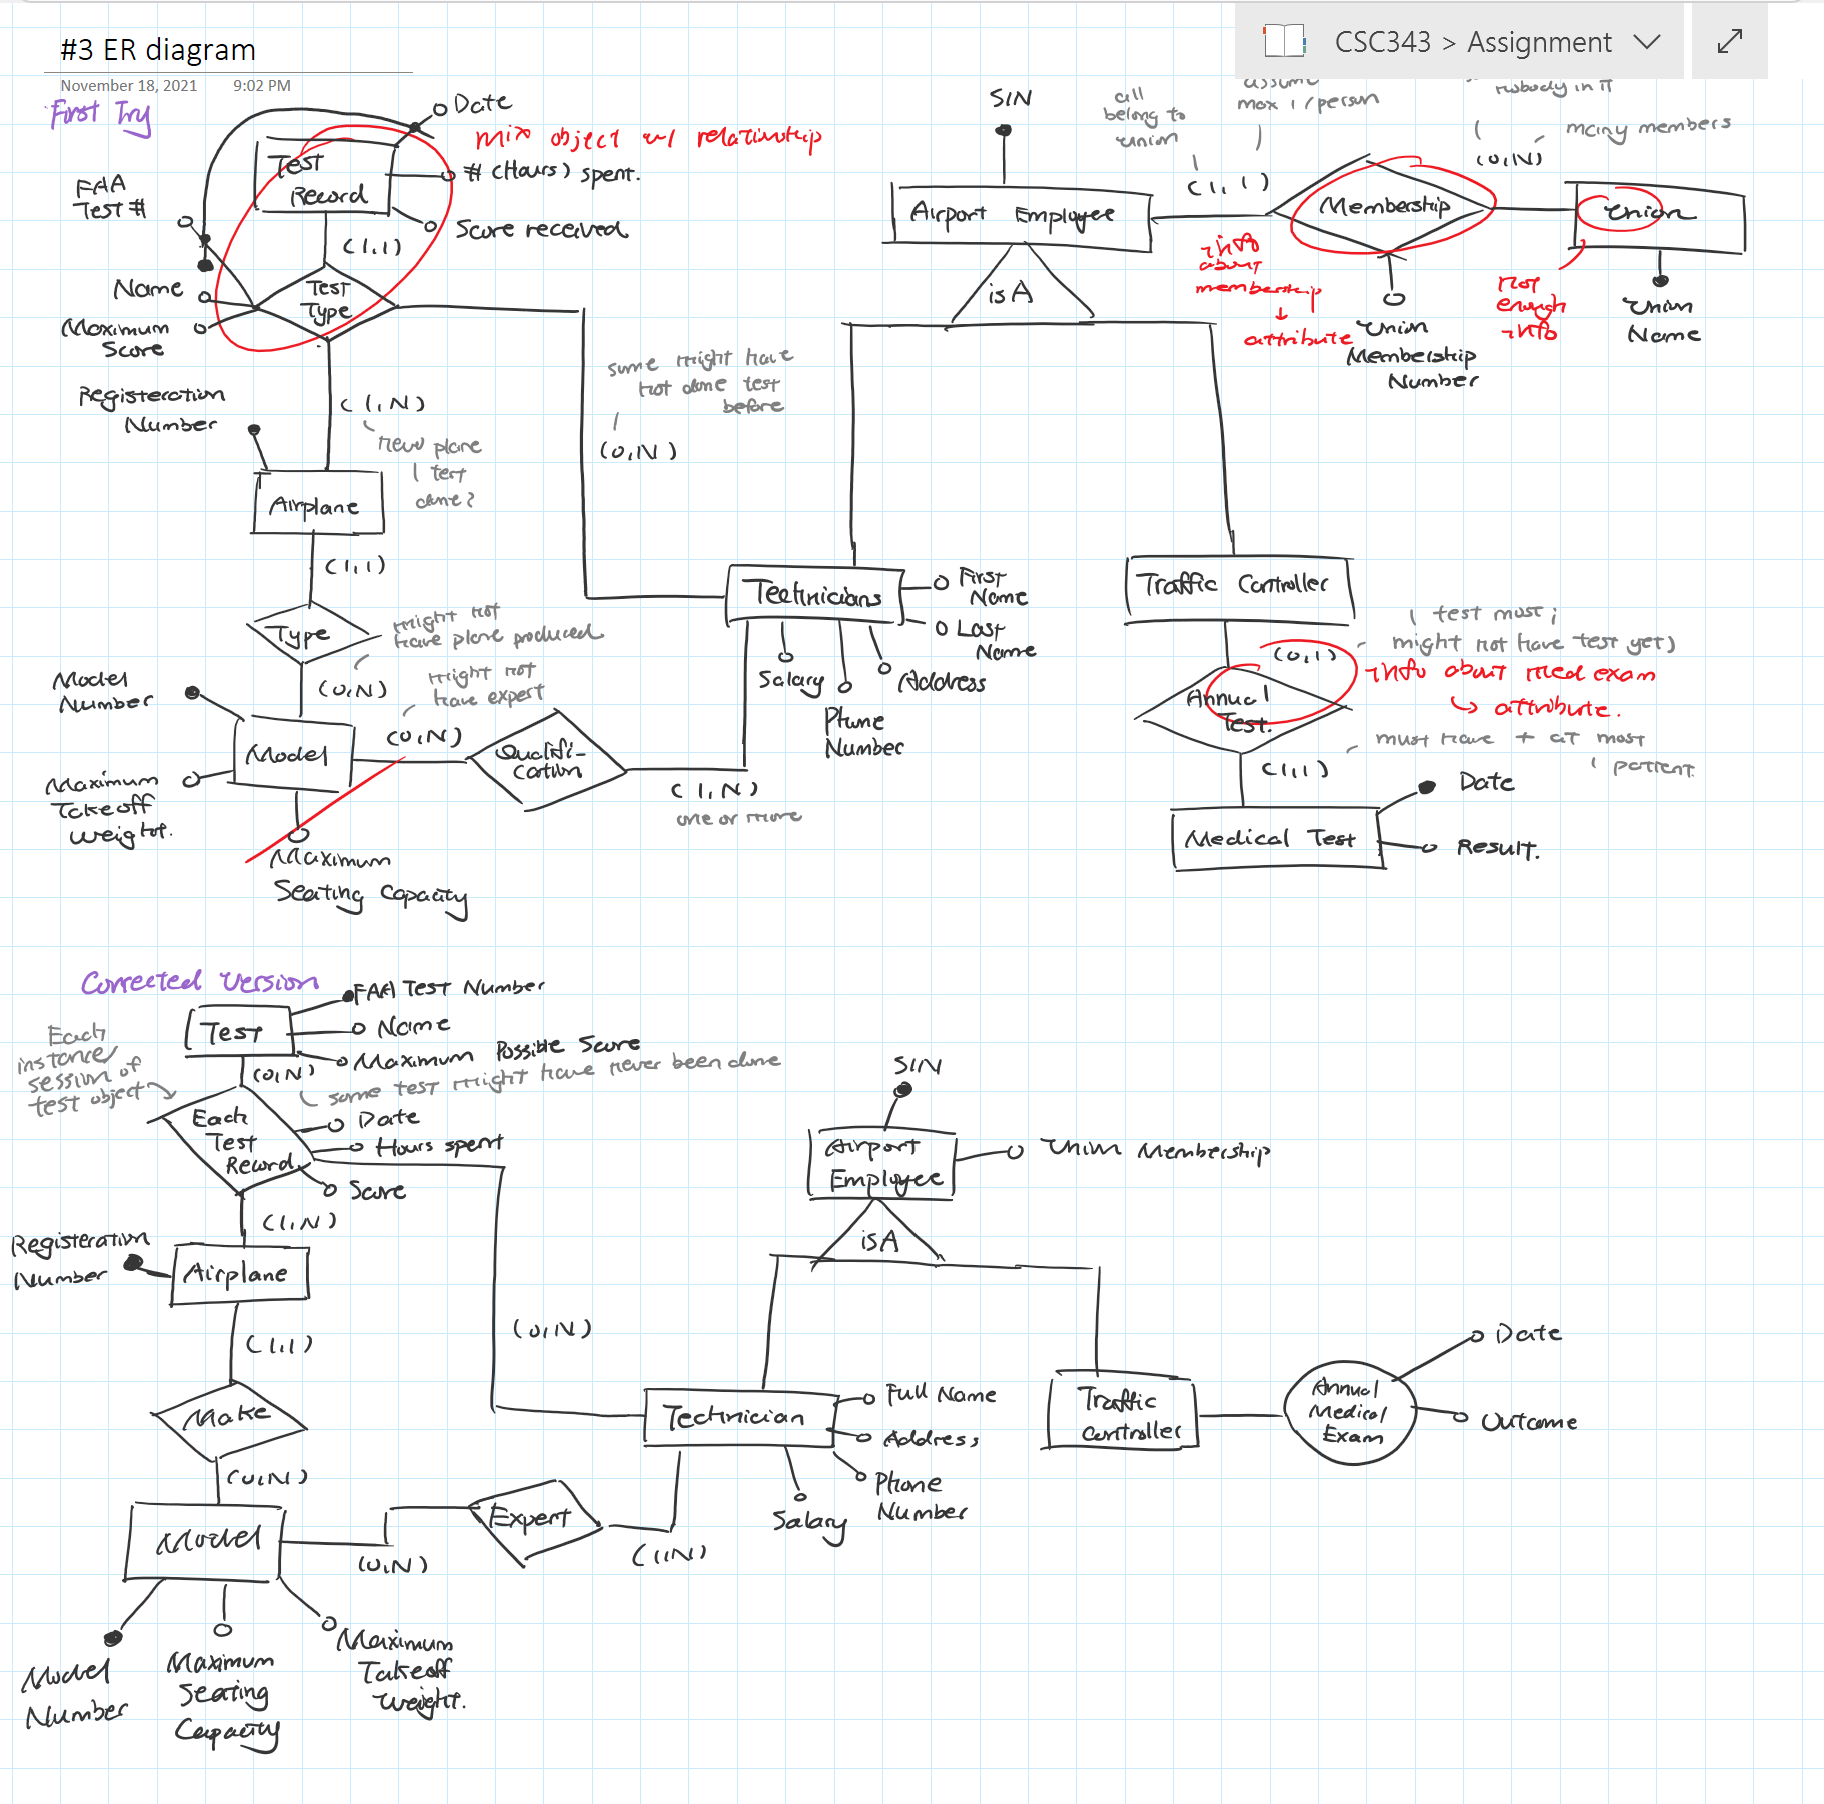
\includegraphics[width=\textwidth]{ER diagram.png}

\end{document}
